% !TeX spellcheck = en_US 
%\documentclass[12pt]{amsart}
\documentclass[varwidth]{standalone}
%\documentclass{standalone}
%\usepackage{amsmath, amsthm, amsfonts, amssymb, latexsym}

% required packages
\usepackage{pgfplots, tikz-3dplot, ifthen}


\begin{document}
	

	\begin{figure}
	\begin{center}
	\begin{tikzpicture}[scale=0.75]
		\draw (-2.828,2.828) -- (2.828,-2.828);  % H_1 
		\draw (2.828,2.828) -- (-2.828,-2.828);  % H_2 
		\draw (-1.,3.872) -- (-1.,-3.872);  % H_3 
		\draw (1.,3.872) -- (1.,-3.872);  % H_4 
		\draw (3.872,-1.) -- (-3.872,-1.);  % H_5 
		\draw (3.872,1.) -- (-3.872,1.);  % H_6 
	\end{tikzpicture}
	
	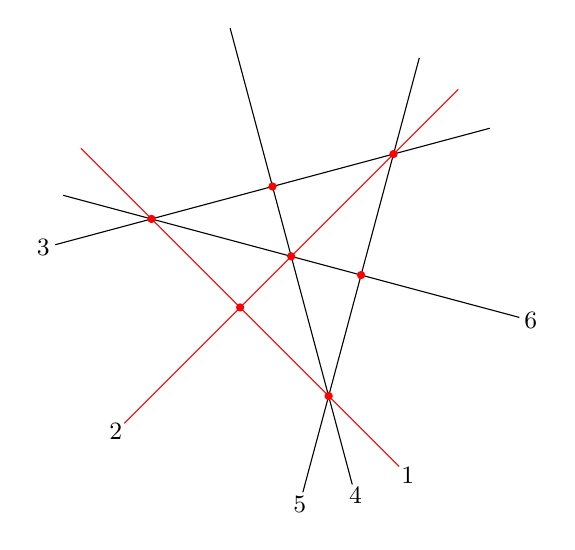
\begin{tikzpicture}[scale=0.75]
		\draw[color=red] (-3.559,1.827) -- (1.827,-3.559);  % H_1 
		\node at (1.975,-3.707) {\small $1$}; 
		\draw[color=red] (2.827,2.827) -- (-2.827,-2.827);  % H_2 
		\node at (-2.970,-2.970) {\small $2$}; 
		\draw (3.361,2.169) -- (-3.995,0.197);  % H_3 
		\node at (-4.198,0.143) {\small $3$}; 
		\draw (-1.034,3.863) -- (1.034,-3.863);  % H_4 
		\node at (1.087,-4.057) {\small $4$}; 
		\draw (2.169,3.361) -- (0.197,-3.995);  % H_5 
		\node at (0.143,-4.198) {\small $5$}; 
		\draw (-3.863,1.034) -- (3.863,-1.034);  % H_6 
		\node at (4.057,-1.087) {\small $6$}; 
		
		\fill[red] (-0.865,-0.865) circle[radius=2pt];  % P[ 1, 2 ] 
		\fill[red] (-2.366,0.634) circle[radius=2pt];  % P[ 1, 3, 6 ] 
		\fill[red] (1.732,1.732) circle[radius=2pt];  % P[ 2, 3, 5 ] 
		\fill[red] (0.634,-2.366) circle[radius=2pt];  % P[ 1, 4, 5 ] 
		\fill[red] (0.0,0.0) circle[radius=2pt];  % P[ 2, 4, 6 ] 
		\fill[red] (-0.317,1.183) circle[radius=2pt];  % P[ 3, 4 ] 
		\fill[red] (1.183,-0.317) circle[radius=2pt];  % P[ 5, 6 ] 
		
	\end{tikzpicture}
	
	\end{center}
	\caption{Example of pictures produced by \texttt{DrawLatex3Arr}.}
	\end{figure}
	
	
	
\end{document}